\section{Chi Squared Test}
In this section, we will talk about Chi Squared Test for homogeneity and for independence. The two tests are the same but the setups are different. In reality, statistics should get involved into the research as early as possible. Nowdays, people sometimes looks for the data and then try to apply statistic models on it because the computational cost is low. However, in the early age of the study, statistics can get involved with the experiment design.

\subsection{Pearson's $\chi^2$ Test for Multinomial Data}
Pearson's $\chi^2$ test is used for multinomial data. Recall that if $X = (X_1, \cdots, X_k)$ has a multinomial($n,p$) distribution, then the MLE of $p$ is $\hat{p} = (\hat{p_1}, \cdots, \hat{p_k}) = (X_1/n, \cdots, X_k/n)$.

Let $p_0 = (p_{01}, \cdots, p_{0k})$ be some fixed vector and suppose we want to test
\[H_0: p=p_0 ~\text{versus}~ H_1: p \neq p_0\]

\begin{definition}[Pearson's $\chi^2$ statistic]
	Pearson's $\chi^2$ statistic is
	\[T = \sum_{j=1}^{k} \frac{(X_j - np_{0j})^2}{n p_{0j}} = \sum_{j = 1}^{k} \frac{(X_j - E_j)^2}{E_j}\]
	where $E_j = \E(X_j) = np_{0j}$ is the expected value of $X_j$ under $H_0$.
\end{definition}

\begin{theorem}Under $H_0$, $T \rightarrow \chi^2_{k-1}$. Hence the test: reject $H_0$ if $T > \chi^2_{k-1, \alpha}$ has asymptotic level $\alpha$. The $p$-value is $\P(\chi^2_{k-1} > t)$ where $t$ is the observed value of the test statistic.
\end{theorem}
\newpage
\subsection{Test of Homogeneity}
\subsubsection{Assumptions}
We have two populations and the sample sizes are fixed. The outcome is random within each population.

\subsubsection{Hypothesis Test}
The homogeneity hypothesis: the chance of success is the same for both populations.

The large-sample two-sided test based on $T$ can also be presented via
Karl Pearson's chi-squared statistic. $T$ is used to check the difference between $p_1$ and $p_2$, to infer the relationship between $\pi_1$ and $\pi_2$. Now we are going to test the difference between the expected table and the observed table.

Suppose the null hypothesis, $H_0: \pi_1 = \pi_2$, is true, then the best estimator  of the common success probability is $p = n_{\cdot 1} / n$. Using this estimator, the expected values of the random quantities $O_{11}$, $O_{12}$, $O_{21}$, and $O_{22}$ can be estimated, respectively by $E_{11}$, $E_{12}$, $E_{21}$, and $E_{22}$, where
\begin{align*}
	E_{11} &= n_{1\cdot} \times p = \frac{n_1 n_{\cdot 1}}{n};\\
	E_{12} &= n_1 \times (1 - p) = \frac{n_1 n_{\cdot 2}}{n};\\
	E_{21} &= n_2 \times p = \frac{n_2 n_{\cdot 1}}{n};\\
	E_{22} &= n_2 \times (1 - p) = \frac{n_2 n_{\cdot 2}}{n}.
\end{align*}

For example, if $H_0: \pi_1 = \pi_2 = 0.5$ is true, then the expected numbers are 
\begin{figure}[H]
	\centering
	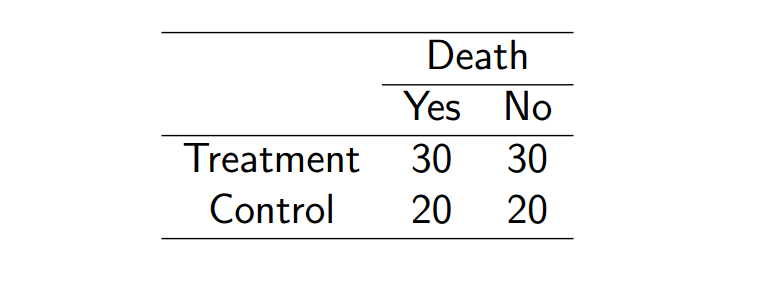
\includegraphics[width=0.7\linewidth]{fig/expected-table}
	\caption{The Exptected Contigency Table}
	\label{fig:expected-table}
\end{figure}

A measure of the discrepancy between the observed frequencies and the estimated exptected frequencies under the hypothesis is the chi-squared statistic
\[S = \frac{(n_{11} - E_{11})^2}{E_{11}} + \frac{(n_{12} - E_{12})^2}{E_{12}} + \frac{(n_{21} - E_{21})^2}{E_{21}} + \frac{(n_{22} - E_{22})^2}{E_{22}}\]

Intuitively, the differences ``observed $-$ expected'', are squared, eliminating the balancing out of positive and negative discrepancies. Each squared difference is weighted by the inverse of the corresponding $E$, so that the difference involving small $E$'s assume the greatest importance.

There is a shortcut formula for the calculation of the chi-squared test statistic, namely,
\[S = \frac{n(n_{11}n_{22}- n_{21}n_{12})^2}{n_{\cdot 1}n_{\cdot 2}n_1 n_2}\]

It can be shown that $T^2 = S$. $S \sim \chi^2_1$, chi-squared distribution with 1 degree of freedom. This implies that the two-sided approximate $\alpha$-level test of $p_1 - p_2 = 0$ versus $p_1 - p_2 \neq 0$, given by the reject region of $|T| \ge z_{\alpha/2}$, is equivalent to the test 
\begin{itemize}
	\item $H_0$: $\pi_1 = \pi_2$.
	\item $H_1$: $\pi_1 \neq \pi_2$. Reject $H_0$ if $S > \chi^2_{\alpha,1}$.
\end{itemize}
\subsubsection{Action in R}
\texttt{chisq.test} is called within \texttt{prop.test}.
\lstinputlisting[language=R]{code/l9-exp4.R}

\subsection{Test of Independence}
\subsubsection{Assumptions}
The main difference in the set-up is that we do not random assign a subject to any group before collecting the data. So that we only have one population, instead of two, but we have four combinations of the result. Therefore, it is meaningful to consider the unconditional probability, i.e. the joint distribution of two factors.
\begin{itemize}
	\item Total sample size $n$ is fixed.
	\item Each observation from a general population is cross-classified on the basis of two factors $X$ and $Y$.
	\item Cell counts are random.
\end{itemize}

\begin{figure}[H]
	\centering
	
\includegraphics[width=0.7\linewidth]{fig/2x2-table2}
	\caption{Example Contingency Table}
	\label{fig:2x2-table2}
\end{figure}

About the contingency table.
\begin{itemize}
	\item The cells are the possible outcomes.
	\item The cell probabilities are the multinomial parameters.
\end{itemize}

Suppose $n_{ij}$ observations in the $ij$-th cell, $i = 1, 2$; $j = 1, 2$.
\begin{figure}[H]
	\centering
	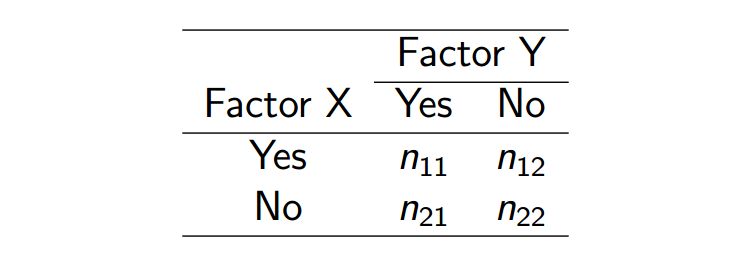
\includegraphics[width=0.5\linewidth]{fig/2x2-table3}
	\caption{Notations in Contingency Table}
	\label{fig:2x2-table3}
\end{figure}

\subsubsection{Hypothesis Test}
Let $\pi_{ij}$ denote the true unknown joint probability of falling into $ij$-th cell, $i = 1, 2$, $j=1,2$. We have
\begin{itemize}
	\item $\pi_{11} = \P(\text{Yes and Yes})$.
	\item $\pi_{12} = \P(\text{Yes and No})$.
	\item $\pi_{21} = \P(\text{No and Yes})$.
	\item $\pi_{22} = \P(\text{No and No})$.
\end{itemize}
The cell probabilities can be represented as follows. 

\begin{figure}[H]
	\centering
	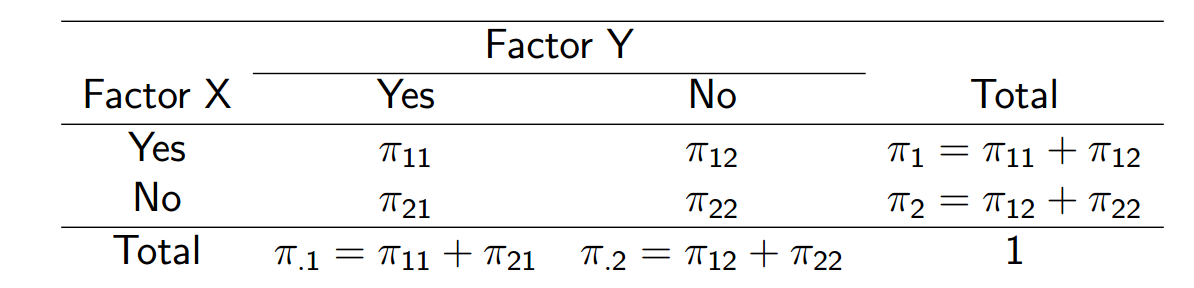
\includegraphics[width=0.7\linewidth]{fig/2x2-table4}
	\caption{Parameters in Contingency Table}
	\label{fig:2x2-table4}
\end{figure}

We would like to set the null hypothesis as that all joint probabilities are equal to the product of their marginal probabilities. So we have
\[H_0: \pi_{ij} = \pi_i \pi_{\cdot j}, i = 1, 2, j = 1, 2\]

Under $H_0$, we have 
\begin{figure}[H]
	\centering
	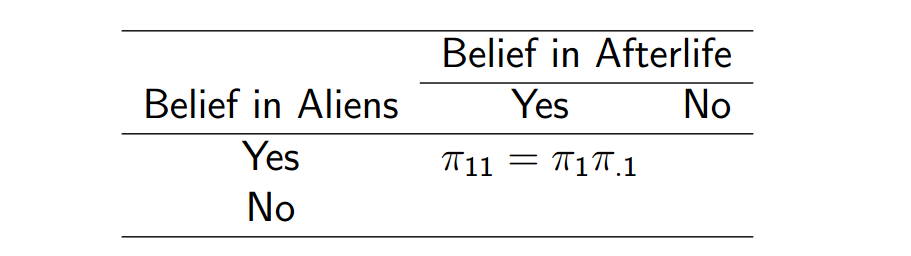
\includegraphics[width=0.7\linewidth]{fig/2x2-table5}
	\caption{Contingency Example under $H_0$}
	\label{fig:2x2-table5}
\end{figure}

The expected value of $n_{11}$ is $n \pi_{11}$, so under the null hypothesis, $n \pi_{11} = n \pi_{1} \pi_{\cdot 1}$.

Moreover, $\pi_1$ can be estimated by $\frac{n_{11} + n_{12}}{n}$ and $\pi_{\cdot 1}$ can be estimated by $\frac{n_{11} + n_{21}}{n}$.

Based on Fig 5, under $H_0$, the estimates of the expected values are
\begin{align*}
	E_{11} &= \frac{(n_{11} + n_{12})(n_{11} + n_{21})}{n};\\
	E_{12} &= \frac{(n_{11} + n_{12})(n_{12} + n_{22})}{n};\\
	E_{21} &= \frac{(n_{11} + n_{21})(n_{21} + n_{21})}{n};\\
	E_{22} &= \frac{(n_{12} + n_{22})(n_{21} + n_{22})}{n}.\\
\end{align*}
The $\chi^2$ test statistics is as follows

\[S = \frac{(n_{11} - E_{11})^2}{E_{11}} + \frac{(n_{12} - E_{12})^2}{E_{12}} + \frac{(n_{21} - E_{21})^2}{E_{21}} + \frac{(n_{22} - E_{22})^2}{E_{22}}\]

We reject $H_0$ if $S \ge \chi^2_{\alpha,1}$.

\subsubsection{Action in R}
\lstinputlisting[language=R]{code/l9-exp5.R}